% fig04_mobius_map.tex
% Mobius map from eccentric exponential z=e^{iG} to complex true anomaly F=e^{if}
\documentclass[tikz,border=5pt]{standalone}
\usepackage{amsmath,amssymb}
\usetikzlibrary{arrows.meta,decorations.pathmorphing,calc,positioning}

\definecolor{accent}{RGB}{0, 100, 170}
\definecolor{highlight}{RGB}{200, 60, 30}
\definecolor{darkgreen}{RGB}{0, 120, 60}
\definecolor{earthblue}{RGB}{40,80,150}
\definecolor{orbitgray}{RGB}{100,100,100}

\begin{document}
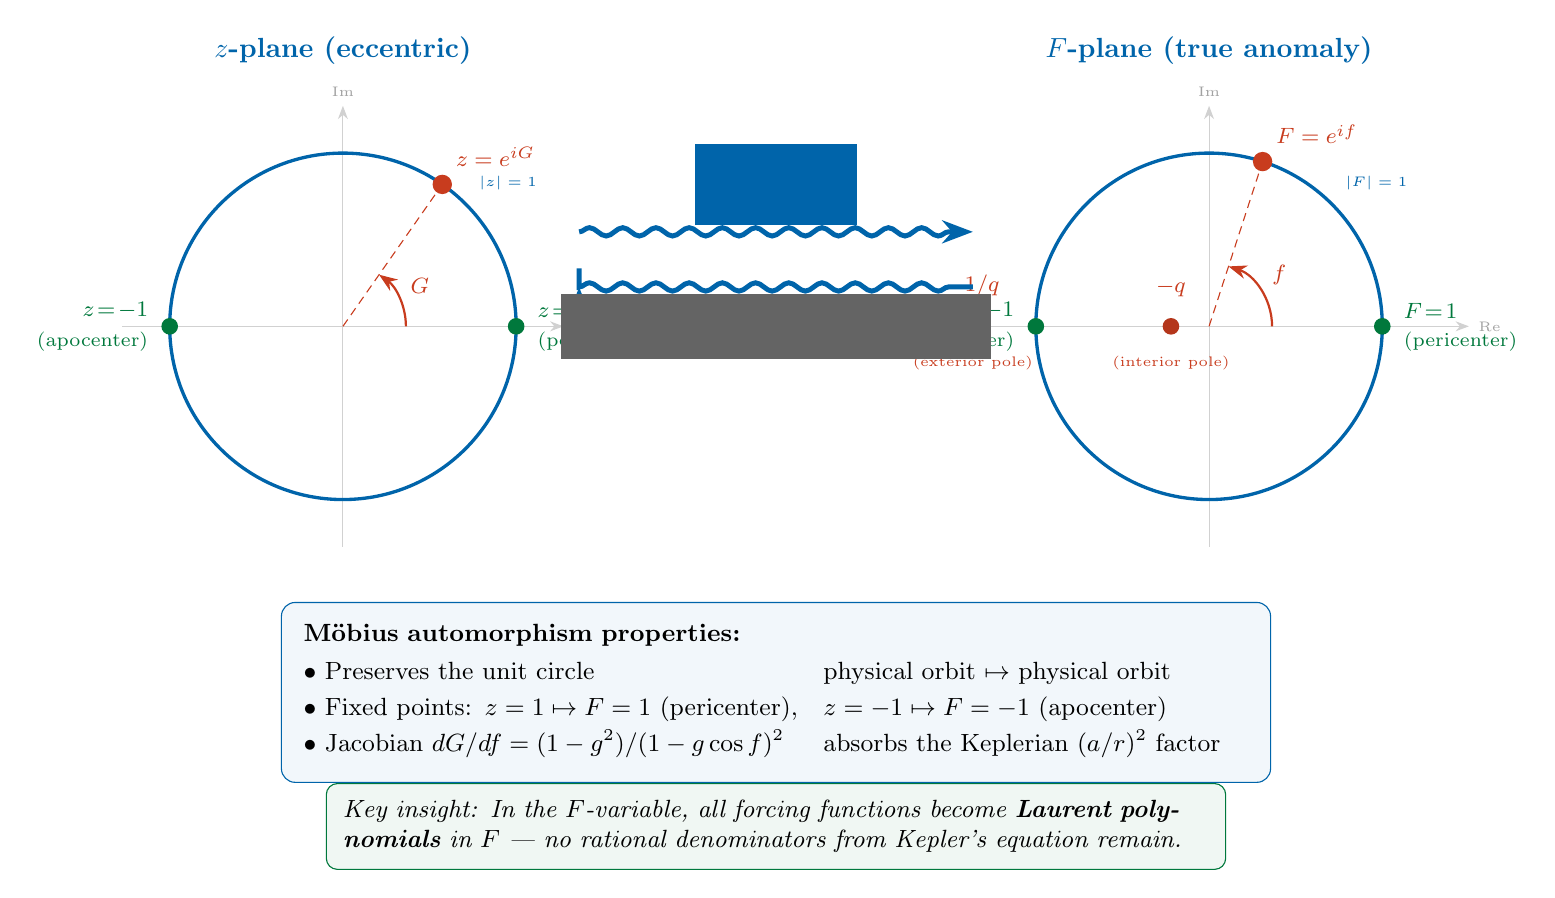
\begin{tikzpicture}[>=Stealth, font=\small]

  % ============================
  % LEFT CIRCLE: z-plane (eccentric)
  % ============================
  \begin{scope}[shift={(-5.5,0)}]

    % Title
    \node[font=\normalsize\bfseries, accent] at (0,3.5) {$z$-plane (eccentric)};

    % Axes
    \draw[orbitgray!30, thin, ->] (-2.8,0) -- (2.8,0)
      node[right, font=\tiny, orbitgray!60] {$\mathrm{Re}$};
    \draw[orbitgray!30, thin, ->] (0,-2.8) -- (0,2.8)
      node[above, font=\tiny, orbitgray!60] {$\mathrm{Im}$};

    % Unit circle
    \draw[accent, line width=1.2pt] (0,0) circle (2.2);
    \node[accent, font=\tiny, anchor=south west] at ({2.2*cos(45)+0.05},{2.2*sin(45)+0.05})
      {$|z|=1$};

    % Pericenter z=1
    \fill[darkgreen] (2.2,0) circle (3pt);
    \node[darkgreen, font=\footnotesize, right] at (2.35,0.2) {$z\!=\!1$};
    \node[darkgreen, font=\scriptsize, right] at (2.35,-0.2) {(pericenter)};

    % Apocenter z=-1
    \fill[darkgreen] (-2.2,0) circle (3pt);
    \node[darkgreen, font=\footnotesize, left] at (-2.35,0.2) {$z\!=\!-1$};
    \node[darkgreen, font=\scriptsize, left] at (-2.35,-0.2) {(apocenter)};

    % Point z = e^{iG} at G=55 degrees
    \pgfmathsetmacro{\Gdeg}{55}
    \pgfmathsetmacro{\zx}{2.2*cos(\Gdeg)}
    \pgfmathsetmacro{\zy}{2.2*sin(\Gdeg)}
    \fill[highlight] (\zx,\zy) circle (3.5pt);
    \node[highlight, font=\footnotesize, above right] at ({\zx+0.05},{\zy+0.1})
      {$z = e^{iG}$};

    % Arc for angle G
    \draw[highlight, thick, ->] (0.8,0) arc[start angle=0, end angle=\Gdeg, radius=0.8];
    \node[highlight, font=\footnotesize] at ({1.1*cos(\Gdeg/2)},{1.1*sin(\Gdeg/2)}) {$G$};

    % Dashed line from origin to z
    \draw[highlight, densely dashed, thin] (0,0) -- (\zx,\zy);

  \end{scope}

  % ============================
  % RIGHT CIRCLE: F-plane (true anomaly)
  % ============================
  \begin{scope}[shift={(5.5,0)}]

    % Title
    \node[font=\normalsize\bfseries, accent] at (0,3.5) {$F$-plane (true anomaly)};

    % Axes
    \draw[orbitgray!30, thin, ->] (-3.3,0) -- (3.3,0)
      node[right, font=\tiny, orbitgray!60] {$\mathrm{Re}$};
    \draw[orbitgray!30, thin, ->] (0,-2.8) -- (0,2.8)
      node[above, font=\tiny, orbitgray!60] {$\mathrm{Im}$};

    % Unit circle
    \draw[accent, line width=1.2pt] (0,0) circle (2.2);
    \node[accent, font=\tiny, anchor=south west] at ({2.2*cos(45)+0.05},{2.2*sin(45)+0.05})
      {$|F|=1$};

    % Pericenter F=1
    \fill[darkgreen] (2.2,0) circle (3pt);
    \node[darkgreen, font=\footnotesize, right] at (2.35,0.2) {$F\!=\!1$};
    \node[darkgreen, font=\scriptsize, right] at (2.35,-0.2) {(pericenter)};

    % Apocenter F=-1
    \fill[darkgreen] (-2.2,0) circle (3pt);
    \node[darkgreen, font=\footnotesize, left] at (-2.35,0.2) {$F\!=\!-1$};
    \node[darkgreen, font=\scriptsize, left] at (-2.35,-0.2) {(apocenter)};

    % Point F = e^{if} — the Mobius map shifts the angle
    % For q ~ 0.22 (e~0.4), f > G; place at about 72 degrees
    \pgfmathsetmacro{\fdeg}{72}
    \pgfmathsetmacro{\Fx}{2.2*cos(\fdeg)}
    \pgfmathsetmacro{\Fy}{2.2*sin(\fdeg)}
    \fill[highlight] (\Fx,\Fy) circle (3.5pt);
    \node[highlight, font=\footnotesize, above right] at ({\Fx+0.05},{\Fy+0.1})
      {$F = e^{if}$};

    % Arc for angle f
    \draw[highlight, thick, ->] (0.8,0) arc[start angle=0, end angle=\fdeg, radius=0.8];
    \node[highlight, font=\footnotesize] at ({1.1*cos(\fdeg/2)},{1.1*sin(\fdeg/2)}) {$f$};

    % Dashed line from origin to F
    \draw[highlight, densely dashed, thin] (0,0) -- (\Fx,\Fy);

    % --- Poles of dM/dF ---
    % Interior pole at F = -q (on negative real axis, inside disk)
    \pgfmathsetmacro{\qval}{0.22}  % q = e/(1+beta) for e=0.4
    \pgfmathsetmacro{\qinv}{1/\qval}  % 1/q ~ 4.55

    % Interior pole
    \fill[highlight!90!black] ({-\qval*2.2},0) circle (3pt);
    \node[highlight, font=\footnotesize, above] at ({-\qval*2.2},0.25) {$-q$};
    \node[highlight, font=\tiny, below] at ({-\qval*2.2},-0.25) {(interior pole)};

    % Exterior pole at F = -1/q (outside disk, on negative real axis)
    \pgfmathsetmacro{\extpole}{-min(\qinv*2.2, 3.0)}  % cap for drawing
    \fill[highlight!90!black] (\extpole,0) circle (3pt);
    \node[highlight, font=\footnotesize, above] at (\extpole,0.25) {$-1/q$};
    \node[highlight, font=\tiny, below] at (\extpole,-0.25) {(exterior pole)};

  \end{scope}

  % ============================
  % CONNECTING ARROW: Mobius map
  % ============================
  \draw[accent, line width=1.8pt, ->,
        decorate, decoration={snake, amplitude=1.5pt, segment length=12pt, post length=6pt}]
    (-2.5,1.2) -- (2.5,1.2);
  \draw[accent, line width=1.8pt, <-,
        decorate, decoration={snake, amplitude=1.5pt, segment length=12pt, post length=6pt}]
    (-2.5,0.5) -- (2.5,0.5);

  % Map formula
  \node[fill=white, inner sep=4pt, font=\normalsize, accent] at (0,1.8) {%
    $\displaystyle F = \frac{z - q}{1 - qz}$%
  };

  % Parameter definition
  \node[fill=white, inner sep=3pt, font=\small, orbitgray] at (0,0.0) {%
    $q = \dfrac{g}{1+\beta}\,,\quad |q|<1\,,\quad
     \beta = \sqrt{1-g^2}$%
  };

  % ============================
  % PROPERTIES BOX (bottom)
  % ============================
  \node[draw=accent, rounded corners=5pt, fill=accent!5,
        inner sep=8pt, text width=12cm, font=\small,
        anchor=north] at (0,-3.5) {%
    \textbf{M\"obius automorphism properties:}\\[3pt]
    \begin{tabular}{@{}l@{\quad}l@{}}
      $\bullet$ Preserves the unit circle &
        physical orbit $\mapsto$ physical orbit \\[2pt]
      $\bullet$ Fixed points: $z=1 \mapsto F=1$ (pericenter),
        & $z=-1 \mapsto F=-1$ (apocenter) \\[2pt]
      $\bullet$ Jacobian $dG/df = (1-g^2)/(1 - g\cos f)^2$ &
        absorbs the Keplerian $(a/r)^2$ factor
    \end{tabular}
  };

  % ============================
  % KEY INSIGHT (bottom annotation)
  % ============================
  \node[draw=darkgreen, rounded corners=4pt, fill=darkgreen!6,
        inner sep=6pt, text width=11cm, font=\small\itshape,
        anchor=north] at (0,-5.8) {%
    Key insight: In the $F$-variable, all forcing functions become
    \textbf{Laurent polynomials} in $F$ --- no rational denominators
    from Kepler's equation remain.
  };

\end{tikzpicture}
\end{document}
